\documentclass{article}
\usepackage{tikz}
\usepackage{geometry}
\usepackage{multicol}

% --- STAFF CONFIGURATION ---
\newcommand{\NumberOfStaves}{24}      
\newcommand{\LineSpacing}{0.2cm}     
\newcommand{\GapBetweenStaves}{1.25cm} 
\newcommand{\StaffThickness}{0.5pt}   

% --- MARGIN CONFIGURATION ---
\newcommand{\MarginTop}{2cm}
\newcommand{\MarginBottom}{2cm}
\newcommand{\MarginLeft}{2cm}
\newcommand{\MarginRight}{2cm}
\newcommand{\ColumnGap}{4cm} 

\geometry{
    a3paper,
    landscape,
    top=\MarginTop,
    bottom=\MarginBottom,
    left=\MarginLeft,
    right=\MarginRight,
    columnsep=\ColumnGap
}

\begin{document}
\pagestyle{empty}

% --- PARAMETER OVERLAY (Does not affect layout) ---
\begin{tikzpicture}[remember picture, overlay]
    \node [anchor=north west, xshift=0.5cm, yshift=-0.5cm, font=\tiny\ttfamily, opacity=0.5] 
    at (current page.north west) 
    {Staves: \NumberOfStaves\ | LineSpacing: \LineSpacing\ | Gap: \GapBetweenStaves\ | Thickness: \StaffThickness};
\end{tikzpicture}

\begin{multicols}{2} 
    \foreach \n in {1,...,\NumberOfStaves}{
        \noindent
        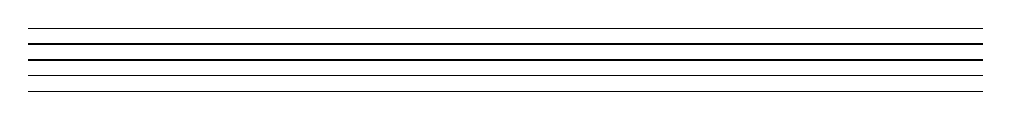
\begin{tikzpicture}
            \foreach \i in {0,1,2,3,4}
            {
                \draw [line width=\StaffThickness] (0, \i*\LineSpacing) -- (\linewidth, \i*\LineSpacing);
            }
        \end{tikzpicture}
        \par
        \vspace{\GapBetweenStaves}
    }
\end{multicols}

\end{document}